\documentclass[sigconf]{acmart}
\settopmatter{printacmref=false} % Removes citation information below abstract
\renewcommand\footnotetextcopyrightpermission[1]{} % removes footnote with conference information in first column
\pagestyle{plain} % removes running headers
\setcopyright{none}

\usepackage{booktabs} % For formal tables
\usepackage[ruled]{algorithm2e} % For algorithms
\renewcommand{\algorithmcfname}{ALGORITHM}
\SetAlFnt{\small}
\SetAlCapFnt{\small}
\SetAlCapNameFnt{\small}
\SetAlCapHSkip{0pt}
\IncMargin{-\parindent}

\usepackage[latin1]{inputenc}
\usepackage{graphicx}
\usepackage{amsmath}
\usepackage{amsfonts}

\DeclareMathOperator*{\argmax}{argmax}

\begin{document}

\title{Entity name extraction from faculty directories}

\author{Jo�o Mateus de Freitas Veneroso}
\affiliation{%
  \institution{Universidade Federal de Minas Gerais}
  \streetaddress{Av. Pres. Ant�nio Carlos, 6627 - Pampulha}
  \city{Belo Horizonte}
  \state{MG}
  \postcode{31270-901}
  \country{Brazil}}
\email{jmfveneroso@gmail.com}

\author{Berthier Ribeiro-Neto}
\affiliation{%
  \institution{Universidade Federal de Minas Gerais}
  \streetaddress{Av. Pres. Ant�nio Carlos, 6627 - Pampulha}
  \city{Belo Horizonte}
  \state{MG}
  \postcode{31270-901}
  \country{Brazil}}
\email{berthier.dcc.ufmg@gmail.com}

\begin{abstract}

Reliable researcher affiliation data is necessary to allow enquiring
about international research group productivity and publication patterns.
Public bibliographic databases such as DBLP and Google Scholar hold
invaluable data about the academic environment. However, the researcher
affiliation information is frequently missing or outdated.
We propose a statistical data extraction method to acquire affiliation 
information directly from university websites and solve the name extraction
task in general.
Previous approaches to web data extraction either lack in flexibility,
because wrappers do not generalize well on cross website tasks, or 
they lack in precision, because domain agnostic methods neglect 
useful properties of this particular application domain.
Our statistical approach solves the name extraction task with 
a framework that incorporates both textual and structural features to
yield an outstanding tradeoff between generality and precision. 
We conducted experiments over a collection of 152 faculty 
web pages in multiple languages from universities in 49 countries
and obtained 94.40\% precision, 97.61\% recall and 0.9597 F-measure at
the extraction task.


\end{abstract}

% \keywords{Information extraction, statistical classifier, web data extraction}

\maketitle

% ==========================================
% Beginning of text.                       |
% ==========================================

\section{Introduction}

Web data extraction is the task of automatically extracting structured information
from unstructured or semi-structured web documents. Typically, Information Extraction 
tasks consist of mapping unstructured or poorly
structured data to a semantically well defined structure. The input is most commonly
composed of a set of documents that describe a group of entities in a similar manner.
The Information Extraction task consists of identifying these entities and 
organizing them according to a template. 

HTML documents most often lie in between the structured / unstructured data paradigm, which means that 
authors take a rather relaxed approach in regard to formal structure. Hierarchy, element disposition,
class names, and other features related to the document structure and indirectly associated
with the data itself are valuable information in the task of identifying entities and 
determining relationships, yet we cannot expect these features to be completely constrained by 
any underlying pattern. Like natural language, organization patterns tend to follow some guidelines 
but are in no way subject to strict rules.

We are interested in the task of name extraction, particularly extracting researcher names from 
university websites to complement data from public databases such as the DBLP repository 
(http://dblp.uni-trier.de/) 
\footnote{
  This is useful, for instance, if one needs to compare the research output of 
  deparments in Germany, or study international publication patterns.
}.
The DBLP database has sparse information about author 
affiliation and only contains information about computer science researchers. We propose
a probabilistic method to handle the name extraction problem in general, without having
to rely on metadata from PDF papers.

\begin{figure}
  \centering
  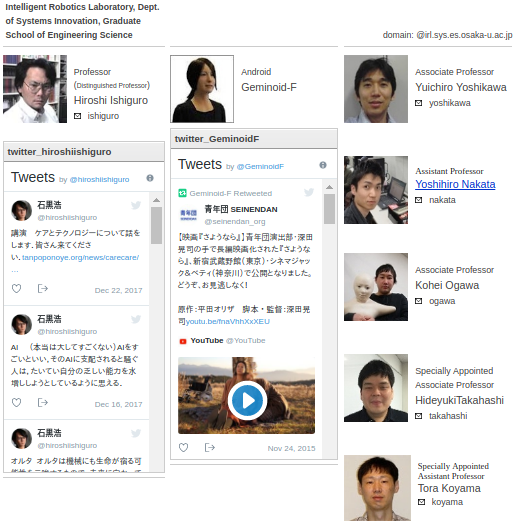
\includegraphics[width=0.5\textwidth]{pics/jap_osaka_lab}
  \caption{Example of a faculty directory}
  \label{fig:faculty_directory}
\end{figure}

To acknowledge the complexity of this extraction task, take for example a snippet of 
the staff page for the intelligent robotics laboratory from Osaka University shown in figure 
\ref{fig:faculty_directory}. There is some structure to the way member profiles are arranged, 
but the organization is rather flexible even considering this single website. Other websites 
can show very different patterns, ranging from tables and lists to free form.

Researcher names can appear inside plain text, similar to typical named entity recognition 
scenarios or in a tabular structure. Names may be part 
of larger sentences such as in "Michael Johnson Chair" and "John 
Doe Avenue" yielding false positives. Names can be composed of common words (e.g. Summer Hall) 
yielding false negatives. There is no rule that fits all cases.

State-of-the-art named entity recognition approaches such as Conditional Random Fields do not 
perform so well in information extraction scenarios such as the one presented in figure 
\ref{fig:faculty_directory}, because the text is insufficient to provide proper contextual 
information about the semantic category of a word. 

A key problem in the task of entity name extraction is accounting for all
possible name combinations. Many names share their spelling with common words, 
or are missing from our database because they are uncommon or unique.
Since we lack a database with all possible name combinations in every language, we propose a 
holistic statistical method that accounts for discrepancies in data organization by assigning 
probabilities to sequences of tokens without relying on per-website training. Our method of
label assignement resembles a Naive Bayesian classifier without the assumption of 
token independence. We also rely as little as possible on contextual information to avoid
the mistakes of other classifiers. The base model already achieves recall and precision rates 
above 90\%, but the performance can be increased even further by incorporating HTML structural
features to estimate better probabilities, especially to avoid filtering out false negatives.


\section{Related Work}

In the last 20 years, the astonishing growth of public information in the web has 
led to the development of a number of different approaches to the problem of web 
data extraction. Traditionally, the task was solved by designing special purpose
programs called wrappers to recognize relevant data and store records in a structured
format. These early tools varied wildly relative to their degree of automation. 

It was readily perceived that manual wrapper generation was a rather tedious and
error prone process, unsuited for large scale operations. Wrappers tend to
break frequently because they rely heavily on web page features that can change 
often. So, in the late nineties, several authors advocated for wrapper induction, a technique 
that consists of automatically constructing wrappers from a small set of examples by 
identifying delimiters or context tokens that single out the desired attributes. 
Some remarkable wrapper induction methods are WIEN \cite{Kushmerick2000}, Soft 
Mealy \cite{Hsu1998} and STALKER \cite{Muslea1999}.

Despite being better than constructing wrappers manually, wrapper induction methods 
still suffered from a lack of expressive power and flexibility. These methods had 
trouble handling records with missing attributes or unusual structures because
patterns could only be identified if they happened at least once in the examples.

Other approaches such as NoDoSE (\cite{Adelberg1998}) and Debye (\cite{Laender2002a}) 
brought greater flexibility to wrapper induction methods by requiring a greater level 
of human interaction through graphical user interfaces. Web data extraction techniques often 
require some sort of assistance from human experts to boost accuracy. One of the main challenges 
in the field lies in determining an adequate tradeoff between the degree of automation and 
the precision and recall of the data extraction tool.

To automate the task of web data extraction completely some approaches,
such as Road Runner \cite{Crescenzi2001}, removed entirely the need for data examples.
Road Runner parses documents belonging to a same class (e.g. books on Amazon) and 
generates wrappers based on their similarities and differences, yielding comparable results 
to those obtained by wrapper induction methods. However like previous approaches, it was 
unsuited for cross site extraction tasks because the learned rules were not general enough.

NLP based approaches aimed at extracting more general rules that could possibly
be employed over multiple websites. RAPIER \cite{Califf1999} is a method of rule
extraction that uses information such as part-of-speech tags and semantic classes from
a lexicon to derive patterns from a set of training examples. This approach is more
flexible than the wrapper induction methods, however it achieves much lower rates of 
recall and precision.

In 2002, a survey by Laender et al. \cite{Laender2002} made a thorough classification of the
early approaches with a taxonomy based on their main technology, being them: languages for
wrapper development, HTML-aware tools, NLP-based tools, Wrapper Induction Tools,
Modeling-based tools and Ontology-based tools. Some noteworthy examples from this era
are: 

\begin{itemize}
\item TSIMMIS \cite{Hammer1997} and WebOQL \cite{Arocena1999}, which are special purpose 
languages for building wrappers.

\item Road Runner \cite{Crescenzi2001}, XWRAP \cite{Liu2000} and W4F \cite{Sahuguet1999}, 
which are HTML-aware tools that infer meaningful patterns from the HTML structure.

\item RAPIER \cite{Califf1999}, SRV \cite{Freitag1998}, WHISK \cite{Soderland1999}, which 
are NLP-based tools.

\item WIEN \cite{Kushmerick2000}, Soft Mealy \cite{Hsu1998} and STALKER \cite{Muslea1999} which 
are wrapper induction methods.

\item NoDoSE \cite{Adelberg1998} and Debye \cite{Laender2002a}, which are semi supervised modeling
based tools that require some interaction with the user by means of a graphical
user interface.
\end{itemize}

In 2006, Chang et al. \cite{Chang2006} complemented the previous surveys with semisupervised 
technologies such as Thresher \cite{Hogue2005}, IEPAD \cite{Chang2001} and 
OLERA \cite{Chang2004}. They differed from supervised 
and unsupervised methods because they either needed only a rough description of
data from users for extraction rule generation or some level of post processing
that needed user attention. The survey also mentioned newer unsupervised methods
such as DeLa \cite{Wang2003}, Exalg \cite{Arasu2003} and Depta \cite{Zhai2005}.

Most of the early information extraction systems were rule-based with either 
manual rule description or automatic rule learning from examples, thus they
suffered from a lack of flexibility when dealing with noisy and unstructured data.
Huge progress in the field of statistical learning led to the development of
statistical models that tried to solve this problem.

In 2008, Sarawagi \cite{Sarawagi2008} produced a survey that classified wrappers in
rule-based methods, statistical methods and hybrid models, bringing together
the fields of named entity recognition, relationship extraction and information
extraction. The rule based methods encompass most of the previous models. The statistical 
methods convert the extraction task into a token labeling task, identifying the 
target entities through the assignment of labels.
Any classifiers such as a Support Vector Machines, Logistic Classifiers or
Neural Networks could be employed to perform this task. However Hidden Markov Models, 
Maximum Entropy Taggers and Conditional Random Fields tend to perform better at most
extraction tasks because of the way they model token and label dependencies. Hybrid models
incorporate both rule-based and statistical methods.

Statistical models have proven to be reliable tools for performing numerous NLP tasks. 
However, information from web documents relevant to data extraction tasks is usually 
arranged in a tabular form rather than in a plain text format. Therefore, typical state
of the art classifiers can yield poor results if they rely exclusively on textual 
information. In the web information extraction task, the document structure must be 
incorporated as a feature in an effective classifier.

More recently, surveys by Ferrara et al. \cite{Ferrara2014} and Schulz et al. \cite{Schulz2016} 
updated the previous surveys with some interesting innovations. Some examples are: the Visual 
Box Model \cite{Krupl2005}, a data extraction system that produces a visualization of 
the web page to exploit visual cues to identify data presented in a tabular form;
automatic wrapper adaptation \cite{Ferrara2011}, a technique that tries to reduce the cost of 
wrapper maintenance by measuring the similarity of HTML trees and adapting
wrappers to the new page structure; AutoRM \cite{Shi2015}, a method to mine
records from a single web page by identifying similar data regions through DOM
tree analysis; and Knowledge Vault \cite{Dong2014}, a method that combines different 
extraction approaches to feed a probabilistic knowledge base.

In 2016, Varlamov et al. \cite{Varlamov2016} argued that the degree of automation can no
longer be the main classification criterion for the data extraction systems
because unsupervised methods which were widely considered to be the state 
of the art when dealing with individual websites performed poorly or were
innapropriate on cross site extraction tasks. The authors proposed a 
classification of methods by the extent of their application. 
The competing approaches were separated into two groups: methods for individual 
websites and methods that are applicable to whole application domains. 

The first group contains most of the earlier approaches, including the supervised
approaches: SRV \cite{Freitag1998}, RAPIER \cite{Califf1999}, WHISK \cite{Soderland1999}, 
WIEN \cite{Kushmerick2000} SoftMealy \cite{Hsu1998} and STALKER \cite{Muslea1999}; and
the unsupervised approaches: RoadRunner \cite{Crescenzi2001} and EXALG \cite{Arasu2003}.

The second group is divided between domain specific methods and domain agnostic methods.
Domain specific methods are designed for extracting data about a particular 
application domain across multiple websites.
Domain specific methods integrate information about the particular application domain in the 
course of its development and thus are able to achieve superior performance in
comparison to domain agnostic methods.
One example is the method of comment extraction 
from blog posts described by Kao et al. \cite{Kao2010}. By incorporating multiple techniques and 
domain specific features they are able to build a classifier that differentiates comment-blocks 
and non-comment blocks. This is only one of many methods tuned for various domains.
Our name extractor method also belongs to this category. 

Domain agnostic methods are the most general extraction methods. They can extract
information from any application domain from multiple websites. They pose the hardest
challenge because the tool must infer data relevance without any prior training in
that particular application domain. Some examples are: ODE (\cite{Su2009}), ObjectRunner 
(\cite{Abdessalem2010}), and AMBER (\cite{Furche2012}). These approaches are more flexible but 
yield worse results than domain specific methods.


\section{Implementation Overview}

The name extraction problem is no different from a Named Entity Recognition problem, however 
approaches that typically achieve high accuracy on NER tasks like Conditional Random Fields, 
Hidden Markov Models or Maximum Entropy Models do not necessarily perform so well when
handling tabular data, as is most common in web data extraction tasks. For example, in 
narrative text, a classifier could learn patterns such as "X spoke to Y" and then discover from 
the sentence "Alice spoke to Bob" that Alice and Bob are names. However in the name extraction task,
the lack of context words prevents these methods from detecting useful patterns over sequences 
of tokens. For instance, tabular data such as the one found in most faculty directories provides 
minimal textual context.

We are also interested in developing a method to extract researcher names regardless of 
the website's main language, even though at this moment we will not be considering non extended-ASCII 
encodings such as Chinese and Farsi characters. Training classifiers over multiple corpora in 
different languages could be in itself a very challenging task. Instead we rely on a priori 
probabilities and structural HTML features to attribute label probabilities to tokens. When manually 
scanning through faculty pages in search of researcher names, the intuitive method to extract them 
is usually identifying a few cases for which we are certain (e.g. Dr. John Smith),
then identifying structural patterns to classify other cases for which we may be not so sure, 
either because they lie outside our knowledge base (e.g. T.J. Bok) or because they sound like
common words (e.g. Summer Hall).


\subsection{Pre-processing}

Before applying the classifier over the web page content, we must run the input web page
through a series of pre-processing steps to clean the data as much as possible.
The HTML document is first parsed producing a DOM tree. At this stage, malformed HTML is
converted into a valid DOM tree as it is commonly done by most browsers nowadays. Header 
details, script tags, style tags, hidden tags and comments are removed. Emails, URLs, and
honorifics are removed through the use of regular expressions.
Spaces, tabs, newlines and special characters are used as separators in a tokenization stage, producing 
a list of tokens. Each token is saved as an object with the following attributes:

\begin{description}
\item [Value:] the token's text in lowercase with converted accented characters.
\item [DOM Element:] a pointer to the DOM Element that contains this token in the DOM Tree.
\item [Previous Token:] the previous token object.
\item [Next Token:] the next token object.
\end{description}

With this simple structure we can extract various features associated with entity names, 
with the benefit of having a list of tokens such as the one we would obtain from a plain 
text format. Through the DOM Element pointer we can figure out the parent elements, nesting 
depth, siblings and other information that can be used to improve estimates in the probabilistic
method we adopt.


\subsection{Name Extraction}

Let $ t = (t_1, t_2, ..., t_n) $ be a sequence of token objects obtained on the pre-processing
stage, and $ y = (y_1, y_2, ..., y_n) $ be a sequence of labels attributed to these tokens
where $ y_i $ can be either a "Name Label" (N), meaning that token $ t_i $ is a person's name, or
a "Word Label" (W), meaning that token $ t_i $ is a common word (not a person's name). Then,
the problem of extracting names from a sequence of tokens is just a series of binary classification 
problems. Considering that each token $ t_i $ has a probability $ P(t_i = y_i) $ of having label 
$ y_i $, the problem of finding an optimal sequence of labels $ y^* $ for a sequence of tokens 
$ t $ can be written as:

\begin{equation}
\\
y^* = \argmax_y P(t_1 = y_1, t_2 = y_2, ..., t_n = y_n)\\
\\
\label{eq:1}
\end{equation}

We may employ the chain rule to explore the relationship between joint and conditional 
probabilities. For ease of exposure, consider that $ P(Y_i) \equiv P(t_i=y_i) $ yielding:

\begin{equation}
\\
P(Y_1, Y_2, ..., Y_n) = P(Y_1) P(Y_2|Y_1) ... P(Y_n|Y_{n-1}, Y_{n-2}, ...)
\\
\label{eq:2}
\end{equation}

A k-gram model could approximate the probabilities $ P(Y_1, Y_2, ..., Y_n) $ by looking
just at the first $ k $ tokens and sliding a window of fixed size $ k $ over the token
sequence. However, the conditional probabilities $ P(Y_i|Y_{i-1}, ...) $ are hard to
estimate, because the joint distribution depends both on the previous labels and the 
previous tokens. If we express them in terms of joint probabilities the problem becomes 
more evident:

\begin{equation}
\\
P(Y_i|Y_{i-1}, Y_{i-2}, ...) \equiv P(t_i, y_i|t_{i-1}, y_{i-1}, t_{i-2}, y_{i-2}, ...)
\\
\label{eq:3}
\end{equation}

To simplify our modeling, let us assume that the probability that token $ t_i $ has label $ y_i $ depends
on the values of previous labels but is independent of the previous tokens. That is, we assume that,
given a sequence of tokens $ \{"John", "Smith"\} $, the conditional probability $ P("Smith"|"John"=Name) $ 
is equivalent to $ P("Smith"|Any\ name) $. In other words, this means that the probability of 
Smith being a last name is the same regardless of a person's first name, as long as we can make sure 
that the previous token is a name. By taking this assumption, Equation \ref{eq:3} becomes:

\begin{equation}
\\
P(Y_i|Y_{i-1}, Y_{i-2}, ...) = P(t_i, y_i|y_{i-1}, y_{i-2}, ...)
\\
\label{eq:4}
\end{equation}

Once again we can employ the chain rule to obtain:

\begin{equation}
\\
P(Y_i|Y_{i-1}, Y_{i-2}, ...) = P(t_i|y_i, y_{i-1}, ...)P(y_i|y_{i-1}, y_{i-2}, ...) \\
\\
\label{eq:5}
\end{equation}

In Equation \ref{eq:5}, the probability $ P(t_i|y_i, y_{i-1}, ...) $ depends on the current and
previous labels. We make a simplifying assumption that $ P(t_i|y_i, y_{i-1}, ...) $ can
be approximated by $ P(t_i|y_i) $. The reasoning behind this is that previous labels have
neglible influence over the particular value of token $ t_i $. For example, we assume that $ P(t_i="John"|t_i=Name) $ 
is a good aproximation for $ P(t_i="John"|y_i=Name, y_{i-1}=Word, ...) $. With this assumption, 
Equation \ref{eq:5} becomes: 

\begin{equation}
\\
P(Y_i|Y_{i-1}, Y_{i-2}, ...) = P(t_i|y_i)P(y_i|y_{i-1}, y_{i-2}, ...) \\
\\
\label{eq:6}
\end{equation}

Finally, by replacing Equation \ref{eq:6} into Equation \ref{eq:2} and grouping together
the second terms of Equation \ref{eq:6} to form the joint probability 
$ P(y_1, y_2, \ldots, y_n) $, we obtain:

\begin{equation}
\\
P(Y_1, \ldots, Y_n) = P(y_1, \ldots, y_n) P(t_1|y_1)P(t_2|y_2) \ldots P(t_n|y_n) 
\label{eq:7}
\end{equation}

Equation \ref{eq:7} can be split into two parts: the prior $ P(y_1, y_2, \ldots, y_n) $
and the conditional token probabilities $ P(t_1|y_1)P(t_2|y_2) \ldots P(t_n|y_n) $.


\subsubsection{Prior probabilities}

The prior probabilities are given by the expression $ P(y_1, y_2, \ldots, y_n) $, which
represents the probability of a series of tokens assuming labels $ \{ y_1, y_2, ..., y_n \} $
without any prior knowledge about the actual token values.

By assuming a window of size $ k \leq n $ we may approximate the priors by calculating the
joint probability $ P(y_1, y_2, \ldots, y_k) $. We observed empirically that when a name 
token is found, it is very likely that the next token will
also be a name. However, arbitrary sequences of non-name tokens do not alter significantly the
probabilities for the next token's label. Put in other words, $ P(y_i|y_{i-1} \neq Name) \approx P(y_i) $.
We can use this property to slide the window of $ k $ tokens over the entire sequence of tokens 
and estimate probabilities without deviating too much from the real distribution. We start at
the beginning of the token list and calculate probabilities for each possible sequence of labels,
taking the most likely one. If the first token is not a name we slide the window right by one token 
and repeat the process. If the first token is a name, then we extract all the tokens that are part of
that name starting from the first one and slide the window right by the number of name tokens extracted. It is
important that the window is at least the number of tokens in the longest name (5 seems to be enough on most 
cases), so we can extract it as a single name.

Let $ N $ be a name label and $ W $ be a word label, then for a window of size $ k $ we 
would need to estimate prior probabilities for all $ 2^k $ possible sequences of labels.
For example, taking a window of size $ 4 $, the sequences would be: 
$ \{W, W, W, W\} $, $ \{W, W, W, N\} $, $ \{W, W, N, W\} $, $ \{W, W, N, N\} $, 
..., $ \{N, N, N, N\} $.

When names occur next to each other there is no way to tell where the first name ends and 
the second one starts. To delimit name boundaries we need to estimate
priors for different sequences of name labels in addition to our previous priors.
Let the first and second name labels be $ N_1 $ and $ N_2 $, respectively. Then,
taking a window of size 4, the prior $ \{N, N, N, N\} $, for example, would expand 
into four different cases: 
$ \{N_1, N_1, N_1, N_1\} $, $ \{N_1, N_1, N_1, N_2\} $, 
$ \{N_1, N_1, N_2, N_2\} $, $ \{N_1, N_2, N_2, N_2\} $.


Most of the times when names happen inside a list they tend to be contained inside a 
single HTML element. Even though this is not always the case, this knowledge can be 
incorporated as an additional piece of evidence in our model. This evidence becomes 
especially useful when we are trying to delimit name boundaries. 

\begin{figure}
  \centering
  
\includegraphics[width=0.5\textwidth]{pics/html_example}
  \caption{Tag transition example}
  \label{fig:html_example}
\end{figure}

A tag transition occurs when a token occurs inside an HTML element and the
next token occurs inside a different HTML element.
Take for example the HTML snippet in figure \ref{fig:html_example} with
the sequence of tokens \{ John, Smith, Professor, Emeritus \}. 
There is a tag transition between the tokens "Smith" and "Professor"
because these consecutive tokens are inside different HTML tags.
Let $ * $ indicate a tag transition in a sequence of tokens, then the label sequence
$ \{ y_1, y_2*, y_3, y_4 \} $,  means that the first two tokens
are contained inside a single HTML element, while the remaining tokens are inside 
a different HTML element. For a window of size 4, we would need to estimate prior 
probabilities with 4 possible tag transitions:
$ \{y_1, y_2, y_3, y_4\} $, $ \{y_1*, y_2, y_3, y_4\} $, $ \{y_1, y_2*, y_3, y_4\} $, $ \{y_1, y_2, y_3*,y_4\} $.
We could estimate sequences with multiple tag transitions inside a window of tokens,
however estimates with a single transition have shown good experimental results. 


\subsubsection{Conditional token probabilities}

The conditional probabilities are given by the second part of equation \ref{eq:7}, that is \\
$ P(t_1|y_1)P(t_2|y_2) \ldots P(t_n|y_n) $.
We need to estimate conditional token probabilities for both labels: names and words.
So we need to know $ P(t_i|N) $, the probability that a name is $ t_i $ and
$ P(t_i|W) $, the probability that a common word is $ t_i $.

For our experiments, the conditional token probabilities were obtained by maximum
likelihood estimation with Laplace smoothing to account for tokens that
didn't occur in the corpus. The $ P(t_i|N) $ probabilities were estimated over a 
collection of approximately 1.5 million author names from the DBLP database. The
$ P(t_i|W) $ probabilities were estimated over a corpus of approximately a hundred thousand documents
obtained by a web crawler that collected university pages. In the latter case 
all names were removed from the corpus in order to keep only non-name tokens.

Conditional token probabilities can be made more precise by incorporating features
in equation \ref{eq:7}. We do that by changing the token conditional 
probabilities to:

\begin{equation}
\\
P(t_i, f_1, f_2, \ldots, f_n|y_i) = P(t_i|y_i)P(f_1|y_i) \ldots P(f_n|y_i)
\\
\label{eq:8}
\end{equation}

where $ f_i $ are features, which are assumed to be independent.
Features can be textual or structural. Textual features take textual
clues from context words and the current token value. An example of textual
feature is the token's length, because names tend to be shorter than common words.
Structural features infer token probabilities based on the surrounding HTML structure.
An example of structural feature is the HTML tag, because names tend to occur inside
the same HTML tags in a given document.


\subsubsection{Secondary estimates}

Structural features that were estimated over the entire corpus ended up 
being too general. HTML structure varies wildly between different websites, 
so we cannot extract useful probabilities looking at the entire collection. 
For example, if all names appear inside a <tr> tag in a given document 
it does not mean that names tend to appear inside <tr> tags rather than any other HTML tag
in other documents. However for that particular document we may be able to identify 
other names and exclude non name tokens by knowing that tokens that occur inside <tr> tags
have a higher probability of being names.

Given that the basic algorithm (without structural features) was able to extract a
satisfactory number of names from a web page with sufficient precision on a first run,
we may estimate probabilities for a structural feature $ P(f_j|y_i) $ by looking at
the extracted names. In fact, since we already attributed a label to every token in the 
web page, we can access the originating DOM element through the token object and estimate
feature probabilities by maximum likelihood, as we did for the token conditional probabilities.
For example, we could easily estimate the probability that a name will occur inside a <div> tag 
$ P(div|Name) $ with this method and incorporate this information as a feature in 
Equation \ref{eq:8} on a next run. Since estimates should get better after a second run,
this method can be repeated multiple times to further increase the algorithm's performance.
This method boosted the algorithm's performance considerably in our experiments, even with a
single secondary run.


\subsubsection{Features}

\begin{table}[h]
  \small
  \begin{center}
    \begin{tabular}{ |l|l|l| }
      \hline
      Id & Feature & Description \\
      \hline
      1  & Token incidence      & How often a token happens in a document         \\
      2  & Token length         & The token's character length                    \\
      3  & First+Second parents & First and second HTML parents combined          \\
      4  & Third parent         & Third HTML parent                               \\
      5  & CSS class name       & Innermost valid CSS class                       \\
      6  & Child number         & The child number relative to the HTML parent    \\
      7  & Nesting depth        & The number of HTML parents up to root           \\
      \hline
    \end{tabular}
  \end{center}
  \caption{Features}
  \label{tab:features}
\end{table}

Table \ref{tab:features} describes the list of features tested in our experiments. 
The third feature "First + Second parents" is the combined tag names of the first and
second HTML elements from leaf to root in the DOM tree, starting from the text node.
This combination yields better results than separate features. The fourth feature is 
the same thing for the third parent. The meaning of the remaining features is self
evident.

Only features that showed some evidence of improvement are being shown here.
The missing features were usually thought to handle specific problems such as
street names that could be confused with a person's name. They involved looking at 
context words, word capitalization, honorifics, etc. However, these trials
were not very productive.

By design, the features were chosen with improvements to recall rather than precision in mind. The reason is that
when a data extractor misses useful results, it becomes hard to obtain that data.
However cleaning bad results is a much simpler task to be carried manually.

\subsection{Experiments}

\begin{table}[h]
  \begin{center}
    \begin{tabular}{ |l|l|l|l| }
      \hline
      Features & Precision & Recall & F-measure \\
      \hline
      None  & 91.71\%          & 91.39\%          & 0.9155          \\ 
      1     & 91.28\% (0.3880) & 93.79\% (0.1836) & 0.9252 (0.3026) \\ 
      2     & 92.00\% (0.4189) & 92.03\% (0.4086) & 0.9201 (0.4042) \\
      1+2   & 91.83\% (0.4660) & 93.90\% (0.1586) & 0.9285 (0.2336) \\
      \hline
    \end{tabular}
  \end{center}
  \caption{Textual features experiment}
  \label{tab:base_model}
\end{table}


The test collection was a set of 152 manually labeled faculty directory web pages from
49 different countries with 11782 researcher names. These names are the target of our 
extraction procedure.
We calculated the precision, recall and f-measures for each modeling variant. All
measures were tested for statistical significance with a one tailed paired T-test in
comparison with the base model, the t-values are presented inside parenthesis next to each measure. 
Results were considered to be significant when the t-value was smaller than 0.05. Statistically
significant results are boldened on all tables. All measures were obtained by the averaged 
results of a 5 fold cross validation run. 

The base model uses only priors with the details already described 
in the last section and token conditional probabilities, but no textual or structural features.
Extracted names were only considered to be correct when they resulted on an exact match with the test data.

Table \ref{tab:base_model} describes the results for the base model incorporating different 
textual features. We considered the variants: (1) base model with no features (our baseline),
(2) base model + feature 1 (token incidence), (3) base model + feature 2 (token length), 
(4) base model + features 1 and 2. Our base model already achieves good results (91.71\% precision, 
91.39\% recall, and 0.9155 F-measure), because it relies on simple but universal probabilities
without making assumptions about data organization or contextual information.
Notice that the textual features produced no statistically significant
improvements in comparison to the base model with no features (the first row).

\begin{table}[h]
  \begin{center}
    \begin{tabular}{ |l|l|l|l| }
      \hline
      Features & Precision & Recall & F-measure \\
      \hline
      3         & 93.43\% (0.1280) & \textbf{96.14\% (0.0361)} & \textbf{0.9477 (0.0475)}  \\
      4         & 93.04\% (0.1965) & 95.67\%         (0.0508)  & 0.9433         (0.0740)   \\
      5         & 93.04\% (0.1781) & 95.50\%         (0.0653)  & 0.9425         (0.0819)   \\
      6         & 92.70\% (0.2307) & \textbf{95.60\% (0.0451)} & 0.9413         (0.0725)   \\
      7         & 92.83\% (0.2374) & \textbf{95.79\% (0.0467)} & 0.9429         (0.0789)   \\
      3 + 5 + 7 & 94.23\% (0.0664) & \textbf{97.14\% (0.0163)} & \textbf{0.9566 (0.0212)}  \\
      \hline
    \end{tabular}
  \end{center}
  \caption{Structural features experiment}
  \label{tab:ne_2}
\end{table}

Table \ref{tab:ne_2} describes the results for the base model with secondary estimates 
calculated over double runs and different combinations of structural features.
We considered the variants: (1) base model + feature 3 (first and second parents),
(2) base model + feature 4 (third parent), (3) base model + feature 5 (CSS class name), 
(4) base model + features 6 (child number), (5) base model + features 7 (nesting depth), 
(6) base model + features 3, 5 and 7. We observe in this experiment that features 
3, 6 and 7 produced statistically significant improvements to recall. Though, features 4 and
5 also produced small T-values of 0.0508 and 0.0653 respectively. 
The secondary estimates strategy was very successful in improving all metrics by
incorporating structural features on the base model. The best variant (features 3, 5 and 7), 
achieved a precision of 94.23\%, recall of 97.14\% and F-measure 0.9566 with statistical
significant improvement to both recall and F-measure.


\begin{table}[h]
  \begin{center}
    \begin{tabular}{ |l|l|l|l| }
      \hline
      \# runs & Precision & Recall & F-measure \\
      \hline
      3 & 94.40\% (0.0525) & \textbf{97.48\% (0.0117)} & \textbf{0.9592 (0.0151)} \\ 
      4 & 94.37\% (0.0544) & \textbf{97.58\% (0.0104)} & \textbf{0.9595 (0.0141)} \\
      5 & 94.40\% (0.0523) & \textbf{97.61\% (0.0100)} & \textbf{0.9597 (0.0135)} \\
      6 & 94.37\% (0.0544) & \textbf{97.61\% (0.0100)} & \textbf{0.9596 (0.0138)} \\
      \hline
    \end{tabular}
  \end{center}
  \caption{Multiple runs experiment}
  \label{tab:ne_plus}
\end{table}

Table \ref{tab:ne_plus} describes the results for the best variant from the previous 
experiments (features 3, 5 and 7) running secondary estimates 3, 4, 5 and 6 times.
We observe that multiple runs on the secondary estimates strategy do not
increase performance significantly. In fact, it reaches a plateau after only 3 to 4
runs. Notice that all variants achieved statistical significant improvements to
recall and F-measure and also got very close to reaching statistical significant
improvements to precision. Further runs were omitted because there was no
change after 6 runs.


\section{Conclusion}

Our name extraction method achieved 94.40\% precision, 97.61\% recall 
and 0.9597 F-measure on a corpus of 152 faculty directory web pages from
49 different countries with 11782 researcher names. 
The model is tuned for the particular problem of name extraction, 
but we believe this result can be generalized to solve other data extraction 
problems. The algorithm is general enough to handle other types of information
extraction tasks without the need for too much tinkering.
The secondary estimates strategy was very successful in further improving the
base model. It can also be remodeled to fit other statistical classifiers since
it does not rely on any particular implementation details of our strategy.


% ==========================================
% End of text.                             |
% ==========================================

% \nocite{*}
\bibliographystyle{unsrt}
\bibliography{bibfile}

\end{document}
